\documentclass[../../dissertation.tex]{subfiles}
\begin{document}

\subsection{Grover}
Like it was seen in section \ref{sec:chapGrover}, Grover's algorithm is a quantum alternative to unstructured search problems. Consider the case of finding element $x_0$ out of an unordered list of size $N$. Worst case scenario, a classical algorithm would need to check every element of the list, requiring $N$ steps.\par
The first stage of Grover's algorithm is to create an uniform superposition of all states in the system
\begin{equation}
	\ket{\Psi_0}  = \frac{1}{\sqrt{N}}\sum_{x=0}^{N-1} \ket{x}.
\end{equation}
Next is the application of the Grover iteration process, which starts with an oracle that adds a negative phase to the solution states
\begin{equation}
        \mathcal{O}\ket{x} = (-1)^{f(x)}\ket{x}.
\end{equation}
This operator can be seen as an identity matrix with negative entries corresponding to the solution states, and the operator can be rewritten as 
%TODO: Reescrever com o somatorio dos estados marcados?
\begin{equation}
	\mathcal{O} = I - 2\sum_{m\in M} \ket{m}\bra{m}.
	\label{eq:groverQiskitOracle}
\end{equation}
where $I$ is the identity matrix and $M$ is a set of solutions where $f(m) = 1$, otherwise it's $0$. The matrix associated with this operator will be
\begin{equation}
	\mathcal{O} = 
	\begin{pmatrix}
		(-1)^{f(0)} & 0 & \cdots & 0\\
	        0 & (-1)^{f(1)} & \cdots & 0\\ 
	        \vdots & 0 &  \ddots & \vdots\\ 
		0 & 0 & \cdots &  (-1)^{f(N-1)}
	\end{pmatrix}.
	\label{eq:oracleMatrixQiskit}
\end{equation}
%TODO: Mencionar que o grover se extende a toda a categoria de problemas que envolvam aquela matriz.
The second part of the iteration is an amplitude amplification process by means of the diffusion operator 
\begin{equation}
        %TODO: Decidir se mantenho os H's.
        \mathcal{D} = (2\ket{\Psi_0}\bra{\Psi_0} - I) = H^{\otimes n}(2\ket{0}\bra{0} - I)H^{\otimes n}.
	\label{eq:groverQiskitDiffusion}
\end{equation}
The unitary operator that describes the Grover iteration process will then be
\begin{equation}
        \mathcal{U} = \mathcal{D}\mathcal{O}.
\end{equation}\par
%TODO: Se calhar desenhar o circuito sem ser no qiskit onde e obvio que se aplicam as cenas varias vezes?
As was shown in section \ref{sec:chapGrover} this iteration process will be done several times, depending on the number of elements. Optimal probability of success finding a single solution will be reached after $\floor{\frac{\pi}{4}\sqrt{N}}$ steps, and $\floor{\frac{\pi}{4}\sqrt{\frac{N}{K}}}$ for $K$ solutions, which is a quadratic gain when compared to the classical case.\par

\begin{figure}[!h]
	\centering
	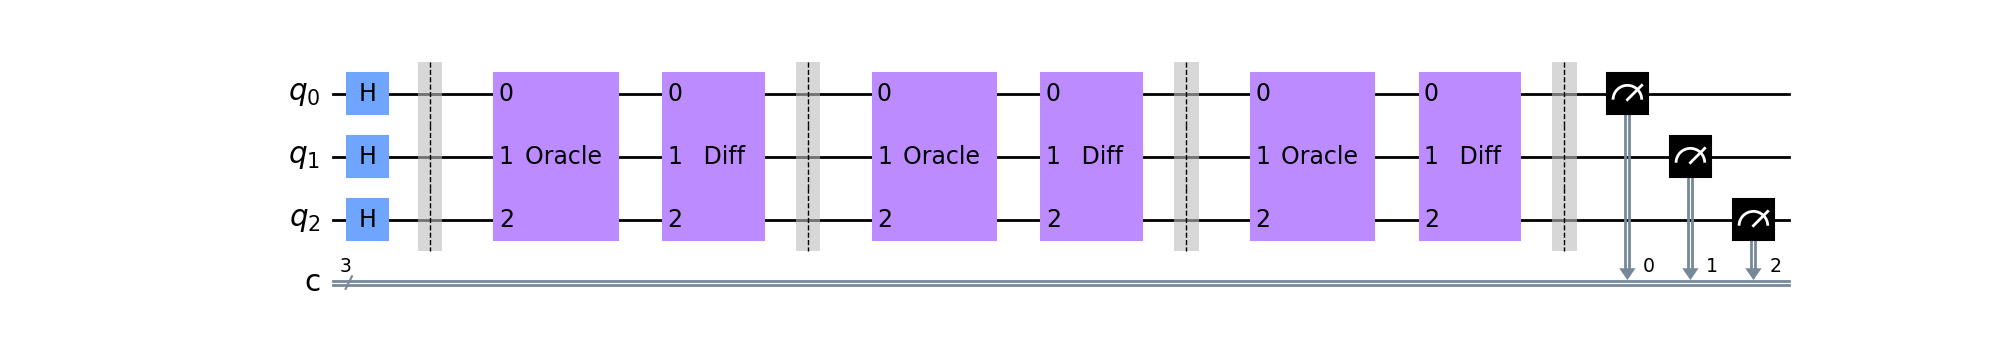
\includegraphics[scale=0.30]{img/Qiskit/GroverQiskit/Circuits/GroverQiskitCirc_N3_M4_S3.png}
	\caption{Temp}
	\label{fig:groverCircuitQistkit}
\end{figure}\par

Consider the $3$ qubit case, where $N=8$ and solution state $\ket{4}$. The optimal number of iterations is approximately $2$, and figure \ref{fig:groverCircuitQistkit} is the circuit for $3$ iterations.
%TODO:Melhorar 
The system starts with the creation of an uniform superposition state, which means applying Hadamard gates to each qubit. 
\begin{figure}[!h]
	\centering
	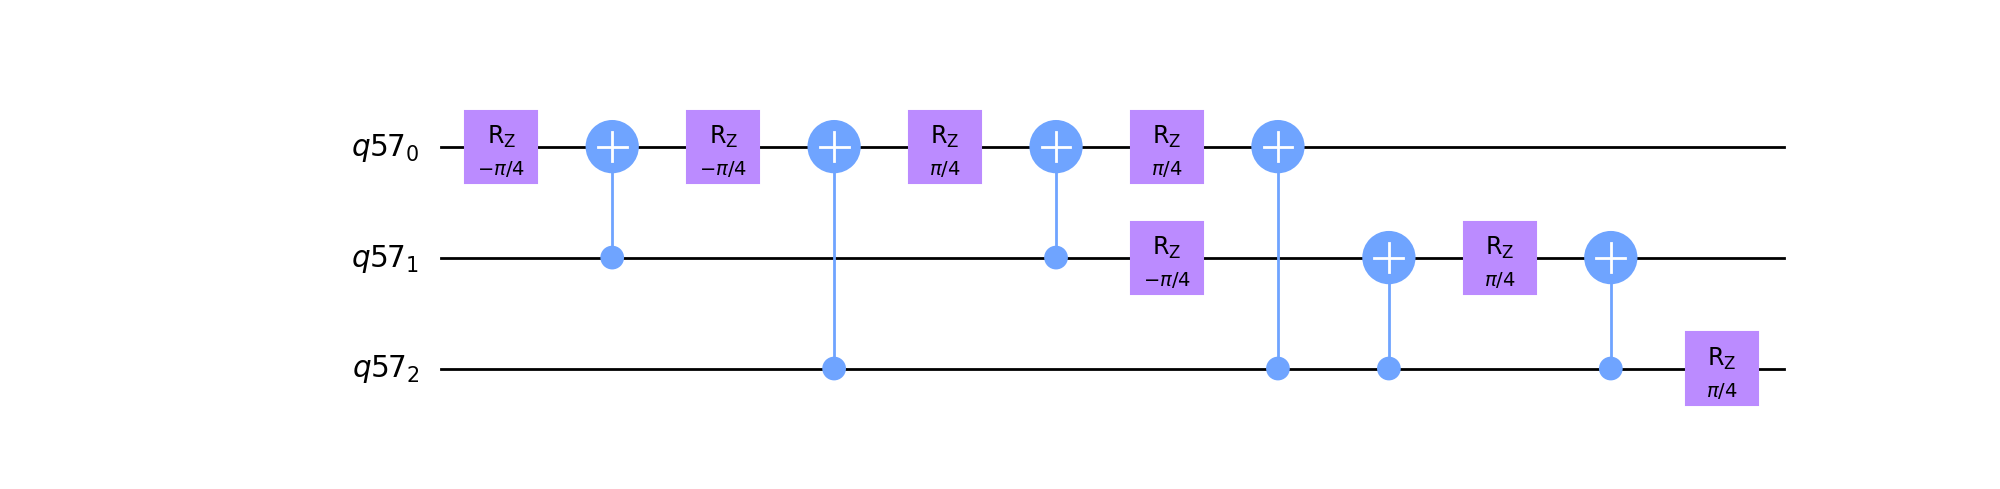
\includegraphics[scale=0.30]{img/Qiskit/GroverQiskit/Circuits/GroverQiskitCircOracle_N3_M4_S3.png}
	\caption{Temp}
	\label{fig:groverOracleCircuitQistkit}
\end{figure}
Immediately following the barrier, the first operator of the iteration process is the oracle, which is shown in figure \ref{fig:groverOracleCircuitQistkit}. 
Because the oracle operator is simply the identity matrix with negative entries corresponding to the solution states, it can be simply translated into a circuit by means of the diagonal function in Qiskit. The last part of the iteration is the diffusion operator, whose circuit is shown in figure \ref{fig:groverDiffCircuitQistkit}.

\begin{figure}[!h]
	\centering
	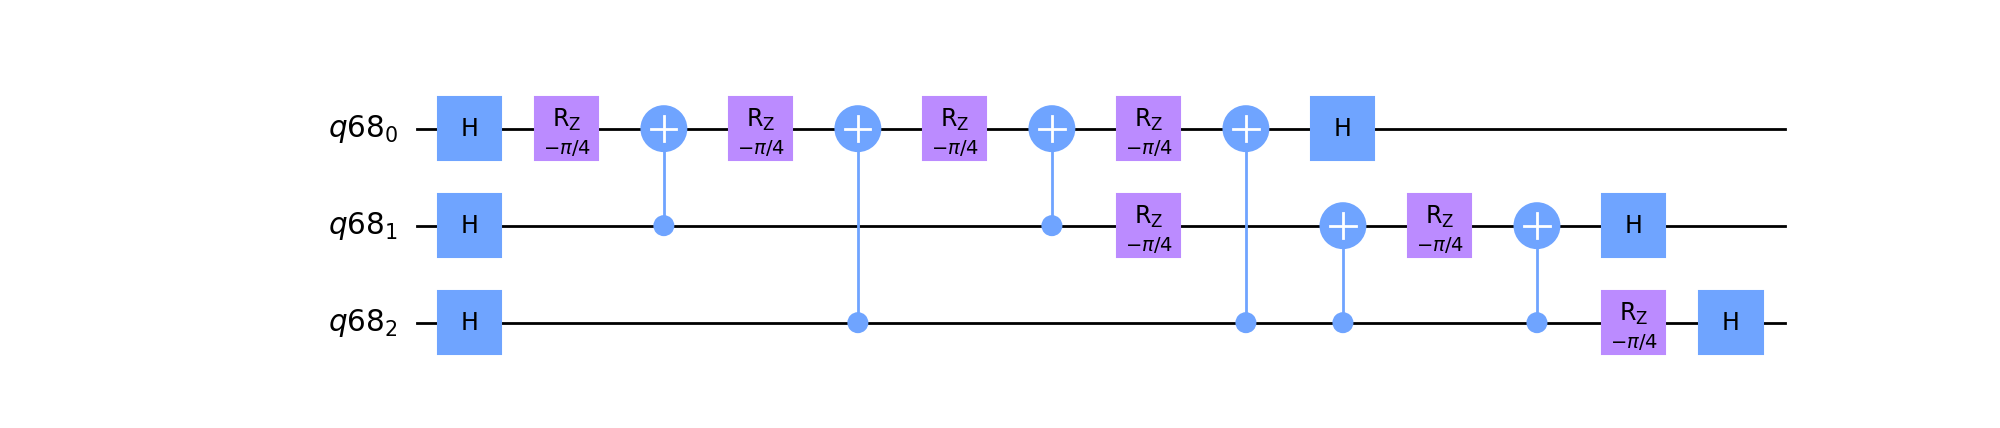
\includegraphics[scale=0.30]{img/Qiskit/GroverQiskit/Circuits/GroverQiskitCircDiff_N3_M4_S3.png}
	\caption{Temp}
	\label{fig:groverDiffCircuitQistkit}
\end{figure}\par
%TODO Isto esta muito fraco. 
Comparing equations \ref{eq:groverQiskitOracle} and \ref{eq:groverQiskitDiffusion}, it is easy to see why figures \ref{fig:groverOracleCircuitQistkit} and \ref{fig:groverDiffCircuitQistkit} are very similar. The diffusion circuit will simply be the oracle circuit for state $\ket{0}$ in between Hadamard operations.


\begin{figure}[!h]
	\centering
	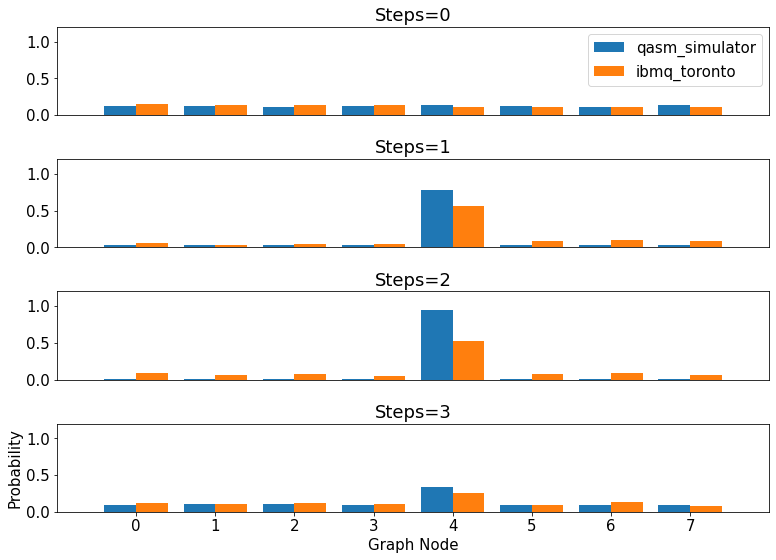
\includegraphics[scale=0.40]{img/Qiskit/GroverQiskit/GroverQiskitSearch_N3_M4_S0123}
	\caption{Temp}
	\label{fig:groverQiskitDist}
\end{figure}
%TODO: Escrever mais
The results of measurement are shown in figure \ref{fig:groverQiskitDist}. As was expected, maximum probability for the marked element was reached after $2$ iterations and it decreases in subsequent steps.

\subsection{Coined}
As previously done in section \ref{sec:chap3CoinedSearch}, this chapter aims to expand the coined quantum walk model incorporating concepts like the oracle and diffusion operator of the Grover algorithm. In fact, for the complete graph case, the coined quantum walk and Grover's algorithm are equivalent.\par
The modified unitary evolution operator is
\begin{equation}
        U' = S (\mathcal{O} \otimes G),\label{eq:modifiedEvoCoinedQiskit}
\end{equation}
%TODO: Relembrar equacoes para cada um dos operadores? Parece me desnecessario.
as was defined in equation \ref{eq:modifiedEvoCoined}, where $S$ is the flip-flop shift operator, $\mathcal{O}$ is the oracle operator and $G$ is the Grover diffusion as a coin operator.\par
Consider the case of a complete graph, where every vertex is adjacent to one another. The quantum circuit to implement this, as shown in figure \ref{fig:coinedSearchCircuit}, will require $N$ qubits to represent the state of the walker and $N$ qubits for the state of the coin.  The shift operator was constructed based on the work of \cite{douglaswang07}, where the state of the walker is flip-flopped with the state of the coin, which can be done through swap gates.
%\begin{figure}[!h]
%	\[ \Qcircuit @C=1em @R=0em { &\qw & \multigate{2}{Oracle} & \qw &\multigate{5}{Shift} & \qw \\
%				     &\qw & \ghost{Oracle} & \qw  & \ghost{Shift} & \qw \\
%               			     &\qw & \ghost{Oracle} & \qw & \ghost{Shift} & \qw \\ 
%				     &\qw & \qw & \multigate{2}{Diff} & \ghost{Shift} & \qw \\
%            			     &\qw & \qw & \ghost{Diff} & \ghost{Shift} & \qw \\ 
%            			     &\qw & \qw & \ghost{Diff} & \ghost{Shift} & \qw  
%		          } \]
%	\centering
%	\caption{Douglas wang coined quantum walk circuit}
%	\label{fig:coinedSearchCircuit}
%\end{figure}
%\begin{figure}[!h]
%	\[ \Qcircuit @C=1em @R=1.0em { &\lstick{\ket{qv}} & {/} \qw &\gate{H^{\otimes n}}  & \gate{O^{\otimes n}} & \qw &\multigate{1}{Shift^{\otimes 2n}} & \qw \\
%				     &\lstick{\ket{qc}}& \qw &{/} \qw & \gate{G^{\otimes n}}& \qw  & \ghost{Shift^{\otimes 2n}} & \qw 
%		          } \]
%	\centering
%	\caption{Douglas wang coined quantum walk circuit}
%	\label{fig:coinedSearchCircuit}
%\end{figure}

\begin{figure}[!h]
	\[ \Qcircuit @C=1em @R=1.0em { &\lstick{\ket{qv}} & {/} \qw &\gate{H^{\otimes n}}  & \gate{O^{\otimes n}} & \qw &\qswap & \qw &\qw  \\
				     &\lstick{\ket{qc}}& \qw &{/} \qw & \gate{G^{\otimes n}}& \qw  &\qswap \qwx& \qw &\qw
		          } \]
	\centering
	\caption{Douglas wang coined quantum walk circuit}
	\label{fig:coinedSearchCircuit}
\end{figure}
%\begin{figure}[!h]
%	\[ \Qcircuit @C=1em @R=2.0em { &\lstick{\ket{qv}} & {/} \qw & \qw & \qswap & \qw &\qw & \qw \\
%				      &\lstick{\ket{qc}} & {/} \qw & \qw & \qswap \qwx & \qw  & \qw & \qw 
%		          } \]
%	\centering
%	\caption{Douglas wang coined quantum walk circuit}
%	\label{fig:coinedSearchShiftCircuit}
%\end{figure}
%
\par
This was implemented in Qiskit, for a graph of size $N=2^3=8$, which means $6$ qubits will be required. For the case of one marked element, the number of iterations that maximizes the amplitude of the solution state is $\floor{\frac{\pi}{2} \sqrt{N}}$, and figure \ref{fig:coinedQWSearchCircuitQistkit}
shows the circuit for 5 iterations of the walk.
\begin{figure}[!h]
	\centering
	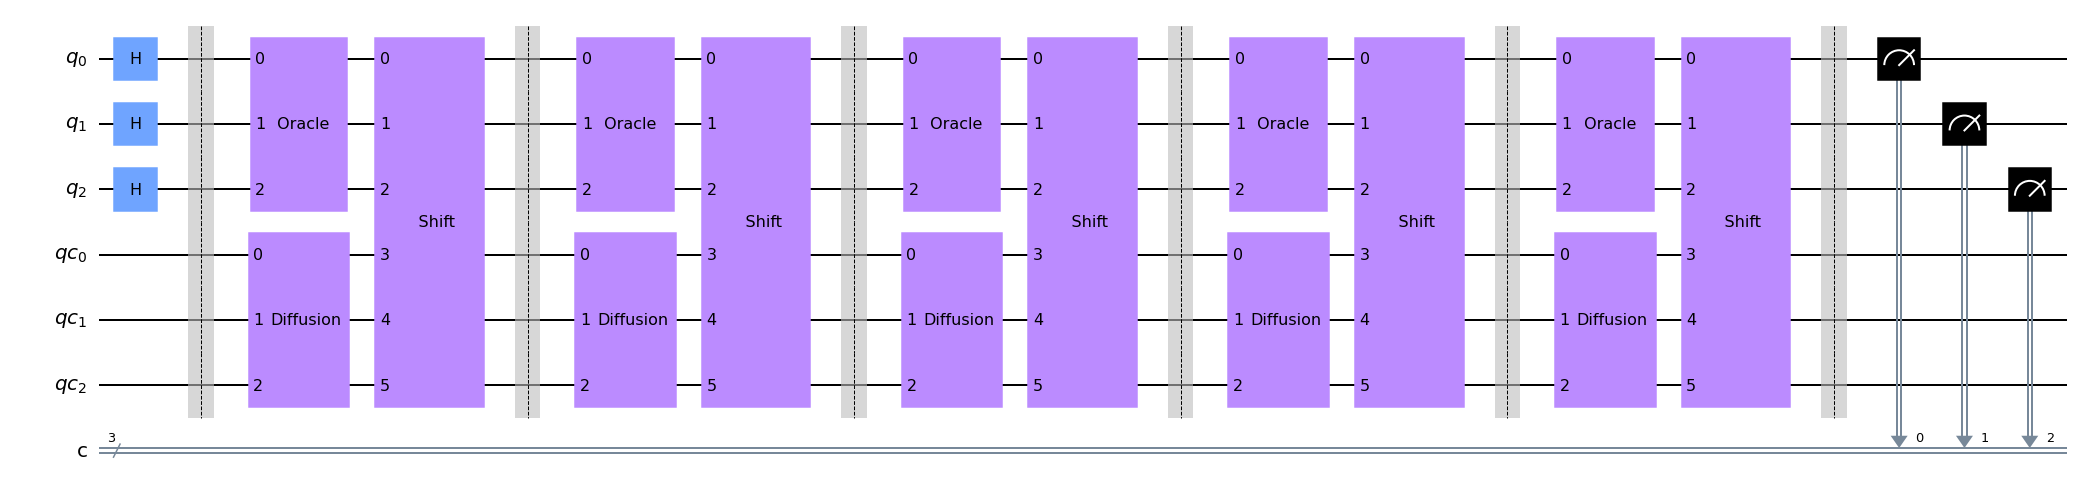
\includegraphics[scale=0.27]{img/Qiskit/CoinedQuantumWalk/Search/Circuits/CoinedSearchQiskitCirc_N3_M0_S5.png}
	\caption{Temp} 
	\label{fig:coinedQWSearchCircuitQistkit}
\end{figure}\par
The circuit starts in a uniform superposition of the states corresponding to the vertices of the graph, and the first step of the iteration is the oracle. This operator will flip the amplitude of the vertex state $\ket{4}$, as is shown in figure \ref{fig:coinedQWSearchOracleCircuitQistkit}. It is the same operator as in figure \ref{fig:groverOracleCircuitQistkit}, but applied only to states belonging in the position space of the walk.

\begin{figure}[!h]
	\centering
	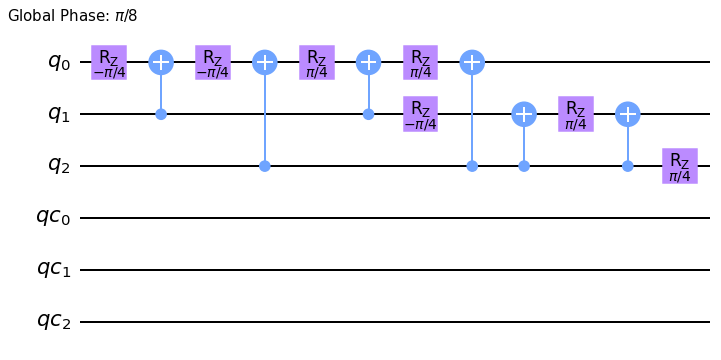
\includegraphics[scale=0.30]{img/Qiskit/CoinedQuantumWalk/Search/Circuits/CoinedSearchQiskitCircOracle_N3_M4_S5.png}
	\caption{Temp} 
	\label{fig:coinedQWSearchOracleCircuitQistkit}
\end{figure}\par
%TODO: Reescrever
The states associated with the coin space of the walk will be transformed according to Grover's diffusion, as is seen in figure \ref{fig:coinedQWSearchDiffCircuitQistkit}.
\begin{figure}[!h]
	\centering
	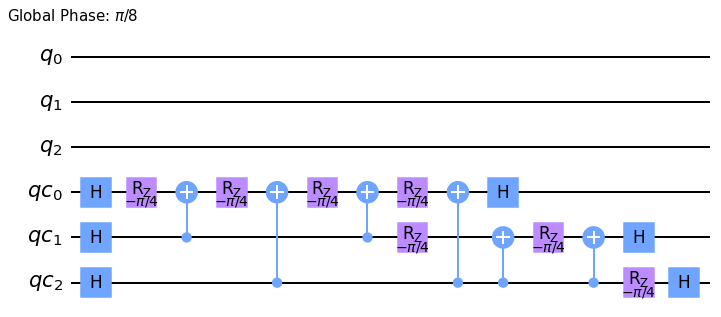
\includegraphics[scale=0.30]{img/Qiskit/CoinedQuantumWalk/Search/Circuits/CoinedSearchQiskitCircDiff_N3_M4_S5.png}
	\caption{Temp} 
	\label{fig:coinedQWSearchDiffCircuitQistkit}
\end{figure}\par
The final part of the iteration is the shift operator, as can be seen in figure \ref{fig:coinedQWSearchShiftCircuitQistkit}. The flip-flop shift operator was defined in equation \ref{eq:chap3FlipFlop} as 
\begin{equation}
        S\ket{v1}\ket{v2} = \ket{v2}\ket{v1},
        \label{eq:chap4FlipFlop}
\end{equation}
where $\ket{v1}$ represents the position of the walker and $\ket{v2}$ is the state of the coin. It is trivial to implement this as shift operations between the vertex states and coin states.
\begin{figure}[!h]
	\centering
	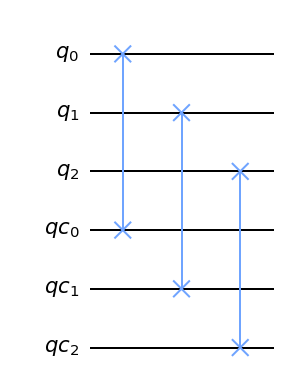
\includegraphics[scale=0.27]{img/Qiskit/CoinedQuantumWalk/Search/Circuits/CoinedSearchQiskitCircShift_N3_M4_S5.png}
	\caption{Temp} 
	\label{fig:coinedQWSearchShiftCircuitQistkit}
\end{figure}\par
%TODO: Estudar porque e que a dist muda logo para 0 (diffusion) em steps = 5
%TODO: Melhorar texto.
Lastly, measurements were performed, and the results plotted in figure \ref{fig:coinedSearchQiskitDist}. Maximum probability of the marked element was reached after $4$ steps, and extra steps reduce said probability. 
\begin{figure}[!h]
	\centering
	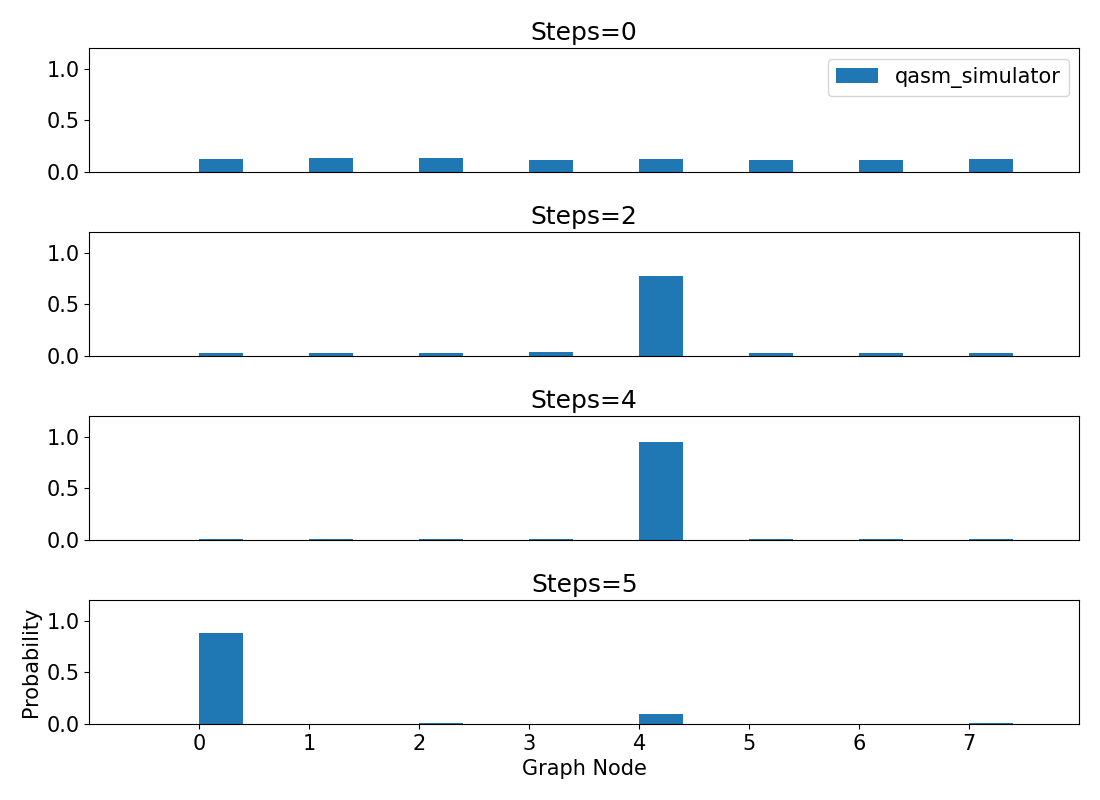
\includegraphics[scale=0.40]{img/Qiskit/CoinedQuantumWalk/Search/CoinedQiskitSearch_N3_M4_S0245}
	\caption{Temp } 
	\label{fig:coinedSearchQiskitDist}
\end{figure}

%TODO: Fazer com outra moeda usando u3 com valores intermedios entre pi/2 ou pi/4
\subsection{Continuous}
As was seen in section \ref{sec:chap3ContSearch}, the unitary operator associated with the continuous time quantum walk model can be modified as to mark an element for amplitude amplification
\begin{equation}
	U'(t) = e^{iH't} = \phi(t)e^{-i\gamma(A+O)t},
	\label{eq:qiskitU'}
\end{equation}
where $\phi(t)$ is a global phase, $A$ is the adjacency matrix and the oracle is defined as 
\begin{equation}
	O = \sum_{m \in M} \ket{m}\bra{m},
\end{equation}
where $M$ is the set of marked elements.\par
%TODO: !!ESCREVER MATRIZ ADJACENCIA GRAFO COMPLETO !!
This section will focus on constructing and analyzing the circuit form of the continuous-time quantum walk search problem, and the first step is to borrow the diagonal definition of the adjacency matrix from equation \ref{eq:qiskitContQWAdj} 
\begin{equation}
    A = F^{\dagger} \Lambda F,
    \label{eq:qiskitContSearchAdj}
\end{equation}
and use the Suzuki-Trotter expansion
\begin{equation}
	e^{i(H_0+H_1)t}=\lim_{n \rightarrow \infty}(e^{i\frac{H_0t}{n}}e^{i\frac{H_1t}{n}})^n ,
\end{equation}
to decompose the operator in equation \ref{eq:qiskitU'}
\begin{equation}
	e^{i\gamma(A+O)t} =\lim_{n \rightarrow \infty}(F^{\dagger} e^{i\gamma\frac{\Lambda t}{n}} F e^{i\gamma\frac{Ot}{n}})^n, 
	\label{eq:suzTrotter}
\end{equation}
which can be easily translated into circuit form as in figure \ref{fig:contSearchCircuit}. 
\begin{figure}[!h]
	\[ \Qcircuit @C=1em @R=1.0em {& & & & & \mbox{Repeat n times} & &\\
	&\lstick{\ket{qv^{\otimes n}}} & {/} \qw &\gate{H^{\otimes n}}  & \gate{e^{i\gamma\frac{Ot}{2}^{\otimes n}}} & \gate{F^{\otimes n}} &\gate{e^{i\gamma\frac{\Lambda t}{2}^{\otimes n}}} & \gate{F^{\dagger}} &\qw \gategroup{2}{5}{2}{8}{.8em}{--}
		          } \]
	\centering
	\caption{Temp}
	\label{fig:contSearchCircuit}
\end{figure}\par
Consider the case of a graph of size $N=3$ and trotter number of $n=2$. The corresponding Qiskit circuit is as shown in figure \ref{fig:contSearchCircuit}. The system starts out in an uniform superposition followed by a state transformation according to the oracle operator that can be seen in figure \ref{fig:contSearchOracleCircQistkit}. Note that the circuit was obtained by using the Qiskit diagonal function that takes the diagonal entries of the operator corresponding to the oracle, as in equation \ref{eq:suzTrotter}. 
\begin{figure}[!h]
	\centering
	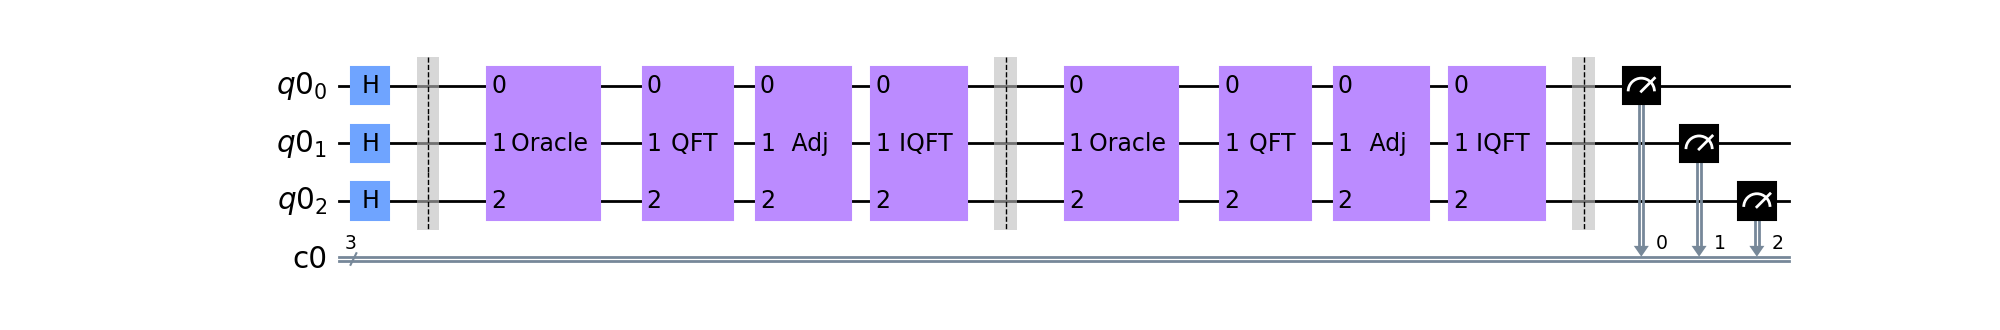
\includegraphics[scale=0.34]{img/Qiskit/ContQuantumWalk/Search/Circuits/circContSearch_N3_S2.png}
	\caption{Temp}
	\label{fig:contSearchCircQistkit}
\end{figure}
%TODO: Escrever mais sobre a adjacencia.
The following transformations will be the quantum Fourier transform, which is the same as in figure \ref{fig:qftCircuitQiskit}, and the operator associated with the adjacency matrix. Since $A$ is the diagonal adjacency matrix of a complete graph, it is easily implemented using Qiskit, as can be seen in figure \ref{fig:contSearchAdjCircQistkit}.
\begin{figure}[!h]
	\centering
	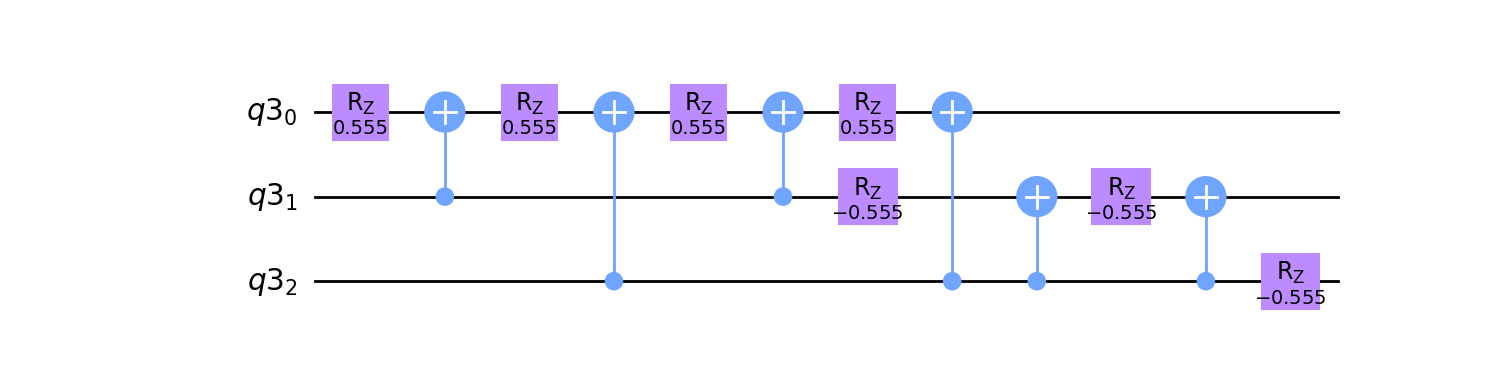
\includegraphics[scale=0.34]{img/Qiskit/ContQuantumWalk/Search/Circuits/circOracle_N3_S2.png}
	\caption{Temp}
	\label{fig:contSearchOracleCircQistkit}
\end{figure}
\par
%TODO: Escrever mais sobre resultados.
The results of measurement are shown in figure \ref{fig:contSearchResultCircQistkit}. 

\begin{figure}[!h]
	\centering
	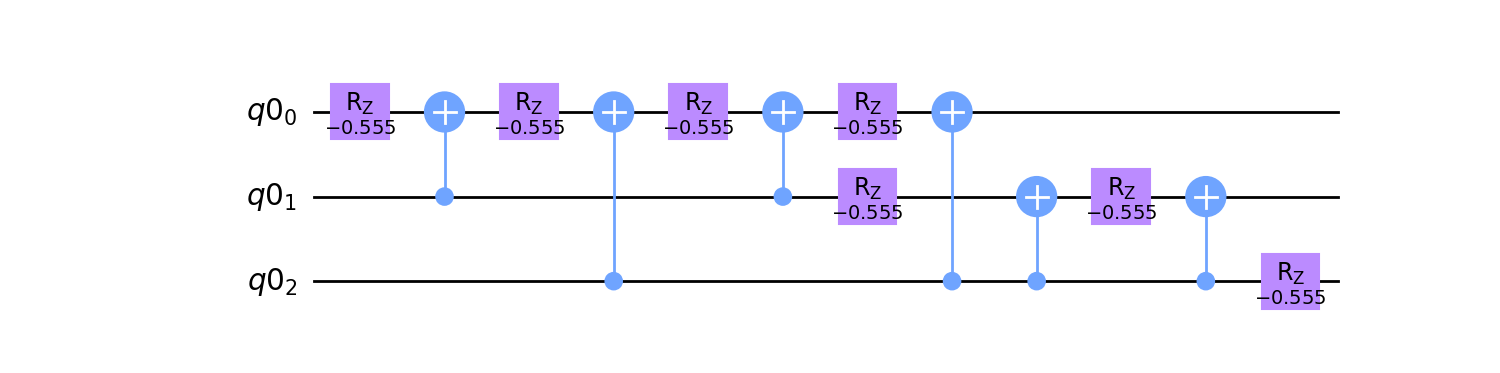
\includegraphics[scale=0.34]{img/Qiskit/ContQuantumWalk/Search/Circuits/circAjd_N3_S2.png}
	\caption{Temp}
	\label{fig:contSearchAdjCircQistkit}
\end{figure}

\begin{figure}[!h]
	\centering
	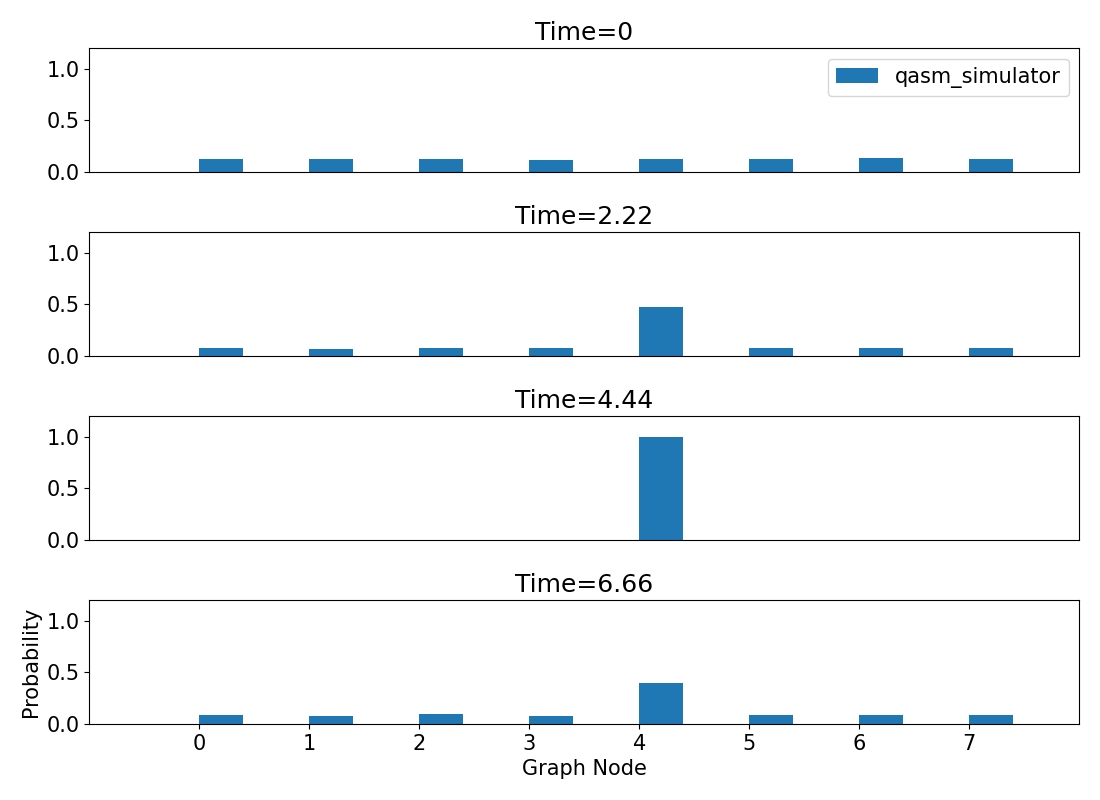
\includegraphics[scale=0.40]{img/Qiskit/ContQuantumWalk/Search/ContQW_N3_S2.png}
	\caption{Temp}
	\label{fig:contSearchResultCircQistkit}
\end{figure}

\subsection{Staggered}
Recalling from section \ref{sec:StagSearchSimul}, the staggered quantum walk on
a complete graph requires a single tessellation with associated polygon
\begin{equation}
	\ket{\alpha} = \frac{1}{\sqrt{N}} \sum_{x=0}^{N-1} \ket{x}.
\end{equation}
The Hamiltonian will then be 
\begin{equation}
	H_\alpha = 2\sum_0^1\ket{\alpha}\bra{\alpha} - I = H^{\otimes n} (2\ket{0}\bra{0} - I) H^{\otimes n} = H^{\otimes n} \mathcal{O}_0 H^{\otimes n},
\end{equation}
which is equivalent to the Grover diffusion operator, meaning it can be
implemented in a similar fashion. The evolution operator for the staggered
quantum walk on the complete graph will then be 
\begin{equation}
	U = e^{i\theta H_\alpha} = e^{i\theta(H^{\otimes n} \mathcal{O}_0 H^{\otimes n})} = H^{\otimes n} e^{i\theta\mathcal{O}_0} H^{\otimes n}.
\end{equation}
This is a very useful representation since the exponent part of the operator is
a diagonal matrix, which means implementing the circuit in Qiskit is a
straightforward task.\par 

Now that the staggered quantum walk associated with the
complete graph is defined, what remains is to add an oracle to the evolution
operator as was done in equation \ref{eq:stagSearchSimulModEvoOp},
\begin{equation}
        U' = U\mathcal{O},
        \label{eq:stagSearchQiskitModEvoOp}
\end{equation}
where
\begin{equation}
	\mathcal{O} = I_N - 2\sum_{m \in M}\ket{m}\bra{m},
\end{equation}
and $M$ is the set of marked elements.\par
The general circuit for implementing the staggered quantum walk search problem
in a complete graph will then be as shown in figure
\ref{fig:stagSearchCircuit}.  
\begin{figure}[!h]
	\[ \Qcircuit @C=1.8em @R=1.5em { &&&& \mbox{Repeat $O(\sqrt{N})$ times.} & &\\
	&\lstick{\ket{\psi_0}} & {/^{\otimes n}} \qw&\gate{\mathcal{O}} &\gate{H}  & \gate{e^{i\theta\mathcal{O}_0}} &  \gate{H} &\qw &\qw \gategroup{2}{4}{2}{7}{.8em}{--} \\
		          } \]
	\centering
	\caption{Temp}
	\label{fig:stagSearchCircuit}
\end{figure}
Since only one tesselation is required, there is no need for the Suzuki-Trotter
aproximation. However, several iterations will be needed in order to achieve
maximum probability for the marked vertex. Because the staggered quantum walk
search on a complete graph is equivalent to Grover's algorithm, the optimum
number of steps will also be $\frac{\pi}{4}\sqrt{\frac{N}{K}}$, where K is the
number of solutions.\par


\end{document}
